\chapter{BVRP previsto e retornos futuros: modelo não linear}
\label{chap:retornos_nao_linear}

Este capítulo repete o teste do Capítulo~\ref{chap:retornos_linear} com um
único modelo em árvore no lugar dos regimes construídos à mão: uma floresta
aleatória, que escolhe sozinha os cortes nas volatilidades, gera o BVRP
previsto, e o retorno futuro é regredido nele. O coeficiente é praticamente
nulo em todos os horizontes, e o teste conjunto nos seis horizontes não
rejeita ($p = 0{,}96$). O resultado se repete com as outras formas e modelos
de previsão e com a floresta aplicada direto ao retorno.

% =========================================================
\section{Especificação}
\label{sec:retnl-especificacao}

A forma principal do BVRP previsto é
\begin{equation}
\widehat{\text{BVRP}}_t = \hat f(X_t) - \text{IV}_t,
\label{eq:retnl-forma}
\end{equation}
em que $\hat f$ é uma floresta aleatória que prevê a volatilidade histórica dos
30 dias seguintes, $\text{VH}_{t+1:t+30}$, com as 17 variáveis $X_t$, as
origens, o embargo e a janela expansiva do Capítulo~\ref{chap:previsao_bvrp}.
Como $\text{BVRP}_t = \text{VH}_{t+1:t+30} - \text{IV}_t$, subtrair a IV de
$t$ da previsão da VH dá uma previsão do prêmio. A floresta entra com todas as
volatilidades em nível e escolhe, em cada divisão, a variável e o ponto de
corte que mais reduzem o erro; os cortes que separam regimes de volatilidade
saem do próprio modelo, sem corte nem variável indicadora fixados de antemão.
A forma~\eqref{eq:retnl-forma} e a floresta foram fixadas antes de ver os
resultados deste capítulo. Como testes de robustez, a floresta prevê o BVRP
diretamente, como no Capítulo~\ref{chap:previsao_bvrp}, e o Ridge é estimado
nas duas formas.

Para cada horizonte $h \in \{1, 5, 10, 20, 30, 60\}$, o retorno simples de
$t$ a $t+h$ é regredido no BVRP previsto, como na
equação~\eqref{eq:met-retorno-linear}, nas mesmas 987 datas fora da amostra e
com a inferência do Capítulo~\ref{chap:retornos_linear}: erro-padrão HAC com
$h+1$ defasagens e bootstrap em blocos em dois níveis, que incorpora a
estimação do BVRP previsto. As reamostragens são as mesmas em todos os
horizontes e nos quatro regressores.

% =========================================================
\section{Previsão do BVRP nas duas formas}
\label{sec:retnl-previsao}

A Tabela~\ref{tab:retnl-previsao} compara as previsões do BVRP. Na forma
$\hat f(X_t) - \text{IV}_t$, a floresta tem $R^2_{\text{fora}}$ de 0,009,
contra 0,143 na forma direta e 0,223 do Ridge direto. A diferença vem da IV. A
forma~\eqref{eq:retnl-forma} impõe coeficiente $-1$ à IV de $t$, e a IV com
coeficiente unitário prevê mal a volatilidade futura: a referência que só usa
a IV, a média histórica da VH menos $\text{IV}_t$, tem $R^2_{\text{fora}}$ de
$-0{,}59$. Na forma direta, o modelo aprende um efeito da IV menor que um. Com
987 datas, porém, o Diebold--Mariano não distingue as duas formas da floresta
($p = 0{,}28$), e no Ridge a diferença fica na fronteira ($p = 0{,}063$). A
variável indicadora do regime de alta volatilidade, acrescentada às
variáveis da floresta, piora a previsão (Diebold--Mariano contra a floresta
sem ela, $p = 0{,}005$).

\begin{table}[H]
\centering
\small
\caption{Previsão do BVRP: forma direta e forma $\hat f(X_t) - \text{IV}_t$.}
\label{tab:retnl-previsao}
\begin{tabular}{lrrrrr}
\toprule
Modelo & $R^2_{\text{fora}}$ & $R^2_{\text{fora}}$ (móvel) & $p$ (CW) & Negativas & BVRP $> 0$ \\
\midrule
Ridge, direta & 0{,}223 & 0{,}095 & $<$0{,}001 & 93\% & $-$5{,}1 \\
Floresta, direta & 0{,}143 & 0{,}073 & $<$0{,}001 & 100\% & $-$6{,}8 \\
Floresta, $\hat f(X_t) - \text{IV}_t$ (principal) & 0{,}009 & $-$0{,}069 & $<$0{,}001 & 67\% & $-$0{,}8 \\
Floresta, $\hat f(X_t) - \text{IV}_t$, com $D_t$ & $-$0{,}041 & -- & $<$0{,}001 & 68\% & $-$1{,}2 \\
Ridge, $\hat f(X_t) - \text{IV}_t$ & $-$0{,}073 & $-$0{,}047 & $<$0{,}001 & 63\% & 0{,}7 \\
Média histórica da VH $-\ \text{IV}_t$ & $-$0{,}588 & $-$0{,}268 & $<$0{,}001 & 25\% & 9{,}8 \\
\bottomrule
\end{tabular}
\par\smallskip
\parbox{0.95\linewidth}{\footnotesize\textit{Nota}: Alvo: $\text{BVRP}_t = \text{VH}_{t+1:t+30} - \text{IV}_t$; 987 previsões, de 21/06/2023 a 03/03/2026. Direta: o modelo prevê o BVRP. $\hat f(X_t) - \text{IV}_t$: o modelo prevê $\text{VH}_{t+1:t+30}$, e a IV de $t$ é subtraída. $D_t$: indicadora do regime de alta volatilidade (corte fixo) como variável a mais. Média histórica da VH $-\ \text{IV}_t$: média de $\text{VH}_{t+1:t+30}$ nos alvos conhecidos na origem, menos a IV de $t$. $R^2_{\text{fora}}$ contra a média histórica do BVRP, nas janelas expansiva e móvel (730 dias); Clark--West unilateral (expansiva), com HAC de 31 defasagens. Última coluna: média do BVRP previsto nas datas em que o BVRP realizado foi positivo, em p.p.}
\end{table}


A forma principal prevê o BVRP pior, mas a conclusão sobre os retornos não
depende dela: as Seções~\ref{sec:retnl-resultados}
e~\ref{sec:retnl-robustez} mostram que nenhuma das quatro combinações de forma
e modelo prevê o retorno.

% =========================================================
\section{Resultados}
\label{sec:retnl-resultados}

A Tabela~\ref{tab:retnl-principal} e a Figura~\ref{fig:retnl-betas}
apresentam os resultados da forma principal. O coeficiente fica entre
$-0{,}076$ e $0{,}070$ p.p. de retorno por p.p. de BVRP previsto, troca de
sinal entre os horizontes, e os valores-$p$ HAC ficam entre 0,55 e 0,94. O
$R^2$ não passa de 0,0014.

\begin{table}[H]
\centering
\small
\caption{Retorno futuro sobre o BVRP previsto pela floresta: estimativas e inferência por horizonte.}
\label{tab:retnl-principal}
\begin{tabular}{rrrrrrr}
\toprule
 & & \multicolumn{3}{c}{HAC} & \multicolumn{2}{c}{Bootstrap em dois níveis} \\ \cmidrule(lr){3-5}\cmidrule(lr){6-7}
$h$ & $\hat\beta_h$ & EP & $p$ & $R^2$ & $\lambda$ & $p$ \\
\midrule
1 & $-$0{,}006 & 0{,}010 & 0{,}553 & 0{,}0003 & 1{,}16 & 0{,}454 \\
5 & $-$0{,}006 & 0{,}038 & 0{,}869 & 0{,}0001 & 1{,}96 & 0{,}757 \\
10 & 0{,}005 & 0{,}066 & 0{,}937 & 0{,}0000 & $-$0{,}35 & -- \\
20 & 0{,}030 & 0{,}136 & 0{,}827 & 0{,}0004 & 0{,}64 & 0{,}904 \\
30 & 0{,}070 & 0{,}209 & 0{,}738 & 0{,}0014 & 0{,}83 & 0{,}801 \\
60 & $-$0{,}076 & 0{,}371 & 0{,}837 & 0{,}0007 & $-$0{,}12 & -- \\
\bottomrule
\end{tabular}
\par\smallskip
\parbox{0.95\linewidth}{\footnotesize\textit{Nota}: $R_{t+h} = \alpha_h + \beta_h\,\widehat{\text{BVRP}}_t + \varepsilon_{t+h}$, com $\widehat{\text{BVRP}}_t = \hat f(X_t) - \text{IV}_t$ e $\hat f$ a floresta aleatória para $\text{VH}_{t+1:t+30}$ (janela expansiva); 987 datas. $\hat\beta_h$ e EP em pontos percentuais de retorno por ponto percentual de BVRP previsto. HAC: Newey--West com $h+1$ defasagens. Bootstrap: 999 reamostragens em blocos de 60 dias; $\lambda$ é a razão entre a média dos $\beta^*$ e $\hat\beta_h$, e o valor-$p$ usa o EP do bootstrap dividido por $\lambda$; com $\lambda \le 0$, a correção não é definida (--).}
\end{table}


\IfFileExists{figs/retornos_nao_linear/fig_betas.png}{
\begin{figure}[H]
    \centering
    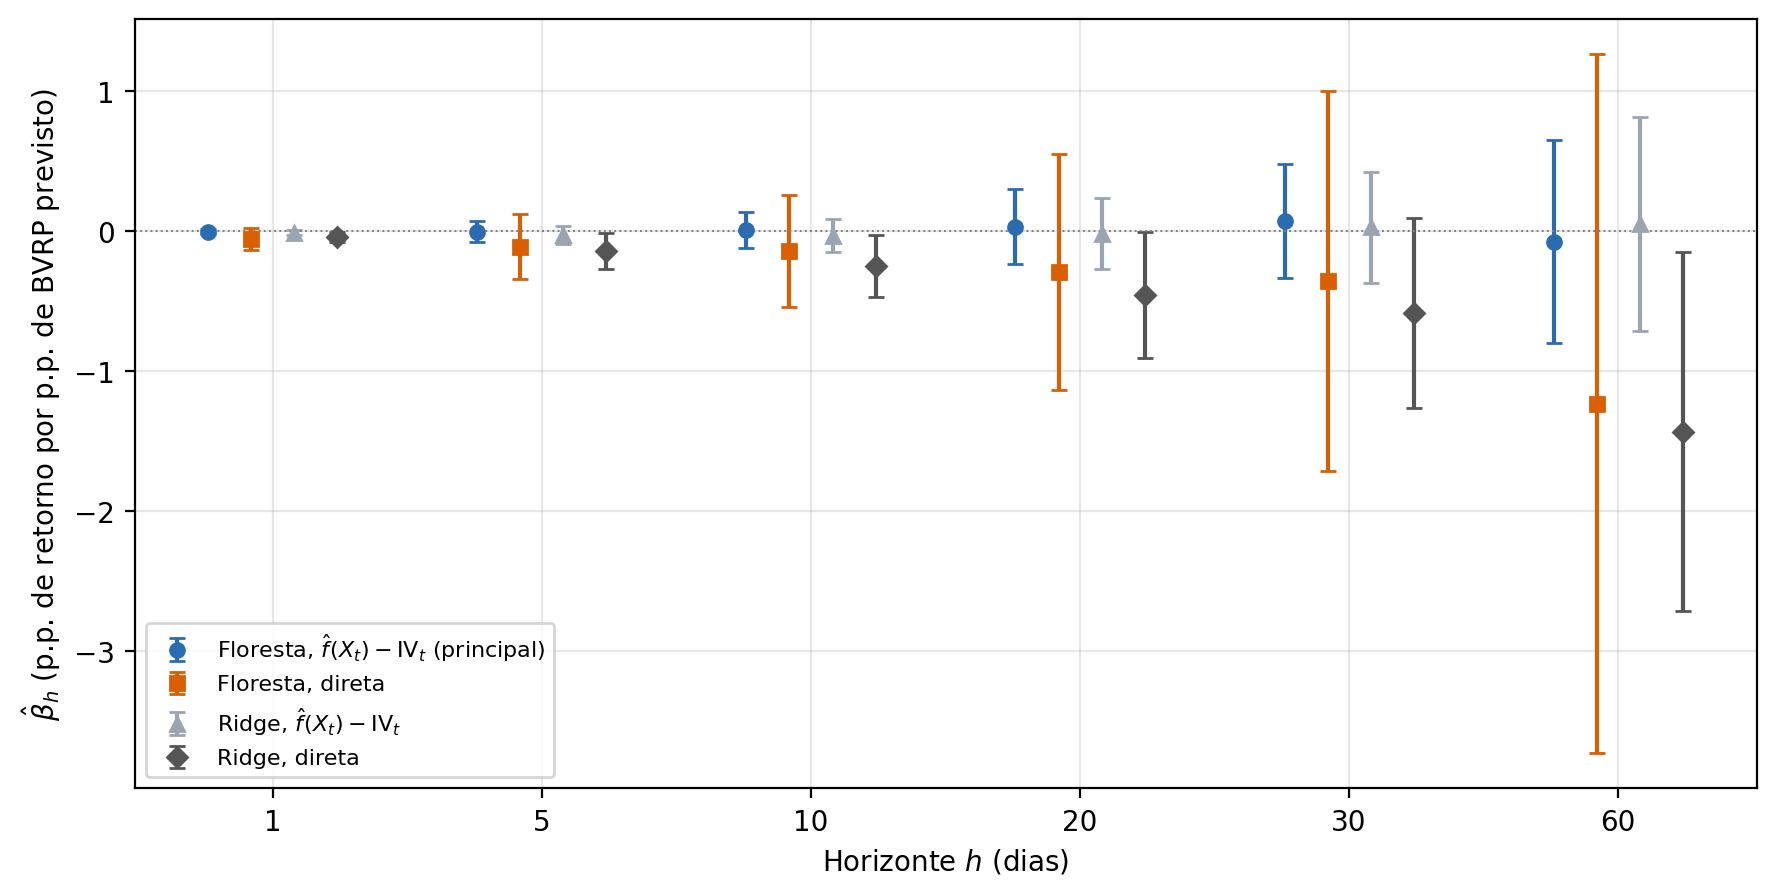
\includegraphics[width=0.9\linewidth]{figs/retornos_nao_linear/fig_betas.png}
    \caption{Coeficiente do retorno futuro sobre o BVRP previsto, por horizonte e regressor, com intervalos de confiança de 95\% pelo erro-padrão HAC com $h+1$ defasagens.}
    \label{fig:retnl-betas}
\end{figure}
}{}

Com $\hat\beta_h$ perto de zero, a correção de escala do bootstrap deixa de
funcionar. A razão $\lambda_h$ entre a média dos $\beta^*$ e $\hat\beta_h$,
que no Capítulo~\ref{chap:retornos_linear} mede a atenuação, divide por um
número próximo de zero: fica entre $-2{,}75$ e $3{,}45$ e é negativa em 5 das
18 combinações de horizonte e tamanho de bloco, casos em que o erro-padrão
corrigido não é definido. Nesses casos, a inferência se apoia no erro-padrão
HAC e no teste conjunto, que não usa $\lambda_h$.

O teste conjunto é um teste de significância conjunta de Wald, cuja
estatística dividida pelo número de restrições é a estatística $F$. Ele testa
$\beta_h = 0$ nos seis horizontes com a covariância dos $\beta^*$ do bootstrap
(Tabela~\ref{tab:retnl-conjunto}). Para a forma principal, $\chi^2(6) = 1{,}45$
e $p = 0{,}96$, e o resultado se repete com blocos de 30 e de 90 dias
($p = 0{,}95$ e $0{,}96$), com o max-$|t|$ ($p = 0{,}79$) e com o HAC das seis
regressões empilhadas ($p = 0{,}93$). Ao contrário do Ridge direto, para o qual
os testes que ignoram a estimação do BVRP previsto rejeitam
(Capítulo~\ref{chap:retornos_linear}), nenhum teste rejeita com a floresta,
nas duas formas.

\begin{table}[H]
\centering
\footnotesize
\caption{Teste conjunto nos seis horizontes.}
\label{tab:retnl-conjunto}
\begin{tabular}{lrrrrr}
\toprule
Regressor & $W$ & \multicolumn{4}{c}{Valor-$p$} \\ \cmidrule(lr){3-6}
 & & Wald & max-$|t|$ & HAC empilhado & só 2º nível \\
\midrule
Floresta, $\hat f(X_t) - \text{IV}_t$ (principal) & 1{,}45 & 0{,}963 & 0{,}791 & 0{,}925 & 0{,}952 \\
\quad blocos de 30 dias & 1{,}63 & 0{,}950 & 0{,}670 & & \\
\quad blocos de 90 dias & 1{,}48 & 0{,}961 & 0{,}905 & & \\
Floresta, direta & 1{,}12 & 0{,}980 & 0{,}708 & 0{,}234 & 0{,}507 \\
Ridge, $\hat f(X_t) - \text{IV}_t$ & 4{,}39 & 0{,}624 & 0{,}382 & 0{,}233 & 0{,}389 \\
Ridge, direta & 6{,}46 & 0{,}373 & 0{,}115 & 0{,}019 & 0{,}032 \\
\bottomrule
\end{tabular}
\par\smallskip
\parbox{0.95\linewidth}{\footnotesize\textit{Nota}: $H_0$: $\beta_h = 0$ nos seis horizontes. Wald: $W = \bar\beta^{*\prime}\,\Sigma^{*-1}\,\bar\beta^*$, com a média e a covariância dos $\beta^*$ do bootstrap em dois níveis (blocos de 60 dias, salvo indicação), $\chi^2(6)$; continua definido quando $\lambda_h \le 0$. max-$|t|$: valor-$p$ global do maior $|z_h|$. HAC empilhado: as seis regressões em conjunto, Newey--West com 61 defasagens. As duas últimas colunas ignoram a estimação do BVRP previsto.}
\end{table}


% =========================================================
\section{Testes de robustez}
\label{sec:retnl-robustez}

A Tabela~\ref{tab:retnl-robustez} repete a regressão com o BVRP previsto pelos
outros três regressores. Com a floresta na forma direta, o coeficiente é
negativo em todos os horizontes, como no Capítulo~\ref{chap:retornos_linear},
mas nenhum é significante (valores-$p$ HAC entre 0,15 e 0,61). Com o Ridge na
forma $\hat f(X_t) - \text{IV}_t$, os valores-$p$ HAC ficam entre 0,12 e 0,90.
O Ridge direto reproduz o Capítulo~\ref{chap:retornos_linear}. O teste conjunto
não rejeita com nenhum dos três quando a estimação do BVRP previsto é
considerada ($p$ entre 0,37 e 0,98).

\begin{table}[H]
\centering
\small
\caption{Testes de robustez: retorno futuro sobre o BVRP previsto por outros modelos.}
\label{tab:retnl-robustez}
\begin{tabular}{lrrrrrr}
\toprule
 & $h = 1$ & $h = 5$ & $h = 10$ & $h = 20$ & $h = 30$ & $h = 60$ \\
\midrule
\multicolumn{7}{l}{\textit{Floresta, direta}} \\
\quad $\hat\beta_h$ & $-$0{,}057 & $-$0{,}113 & $-$0{,}142 & $-$0{,}294 & $-$0{,}357 & $-$1{,}235 \\
\quad $p$ HAC & 0{,}148 & 0{,}342 & 0{,}487 & 0{,}493 & 0{,}606 & 0{,}333 \\
\quad $p$ bootstrap & 0{,}438 & 0{,}597 & 0{,}770 & 0{,}794 & 0{,}834 & 0{,}720 \\
\multicolumn{7}{l}{\textit{Ridge, $\hat f(X_t) - \text{IV}_t$}} \\
\quad $\hat\beta_h$ & $-$0{,}013 & $-$0{,}027 & $-$0{,}034 & $-$0{,}019 & 0{,}024 & 0{,}047 \\
\quad $p$ HAC & 0{,}122 & 0{,}395 & 0{,}580 & 0{,}883 & 0{,}904 & 0{,}904 \\
\quad $p$ bootstrap & 0{,}183 & 0{,}602 & 0{,}905 & -- & 0{,}707 & 0{,}787 \\
\multicolumn{7}{l}{\textit{Ridge, direta}} \\
\quad $\hat\beta_h$ & $-$0{,}045 & $-$0{,}144 & $-$0{,}250 & $-$0{,}459 & $-$0{,}586 & $-$1{,}433 \\
\quad $p$ HAC & 0{,}011 & 0{,}025 & 0{,}029 & 0{,}046 & 0{,}091 & 0{,}028 \\
\quad $p$ bootstrap & 0{,}043 & 0{,}080 & 0{,}170 & 0{,}242 & 0{,}303 & 0{,}143 \\
\bottomrule
\end{tabular}
\par\smallskip
\parbox{0.95\linewidth}{\footnotesize\textit{Nota}: Mesma especificação da Tabela~\ref{tab:retnl-principal}, com o BVRP previsto por outros modelos. Forma direta: previsões do Capítulo~\ref{chap:previsao_bvrp}. Bootstrap em dois níveis, 999 reamostragens em blocos de 60 dias, as mesmas em todos os regressores; -- quando $\lambda \le 0$.}
\end{table}


% =========================================================
\section{Como a árvore escolhe as quebras}
\label{sec:retnl-quebras}

A Figura~\ref{fig:retnl-importancia} mostra a importância das variáveis nas
duas formas da floresta, pela redução de impureza dentro da amostra, média
das 33 origens, e pelo aumento do erro quadrático médio fora da amostra
quando a variável é permutada. Na forma direta, a volatilidade histórica dos
30 dias anteriores é a variável mais importante pelos dois critérios, seguida
da de 90 dias. Na forma $\hat f(X_t) - \text{IV}_t$, a previsão do BVRP é
dominada pela IV, que entra com coeficiente $-1$ por construção, e pela
$\text{BVRP}^{\text{proxy}}_t$, as duas variáveis cuja permutação mais aumenta
o erro. Dentro do modelo da VH, a volatilidade histórica de 90 dias tem a
maior redução de impureza (0,39), mas importância negativa por permutação fora
da amostra: permutá-la reduz o erro. A variável que a floresta mais usa
dentro da amostra não ajuda fora dela, o que é coerente com o
$R^2_{\text{fora}}$ baixo dessa forma.

\IfFileExists{figs/retornos_nao_linear/fig_importancia.png}{
\begin{figure}[H]
    \centering
    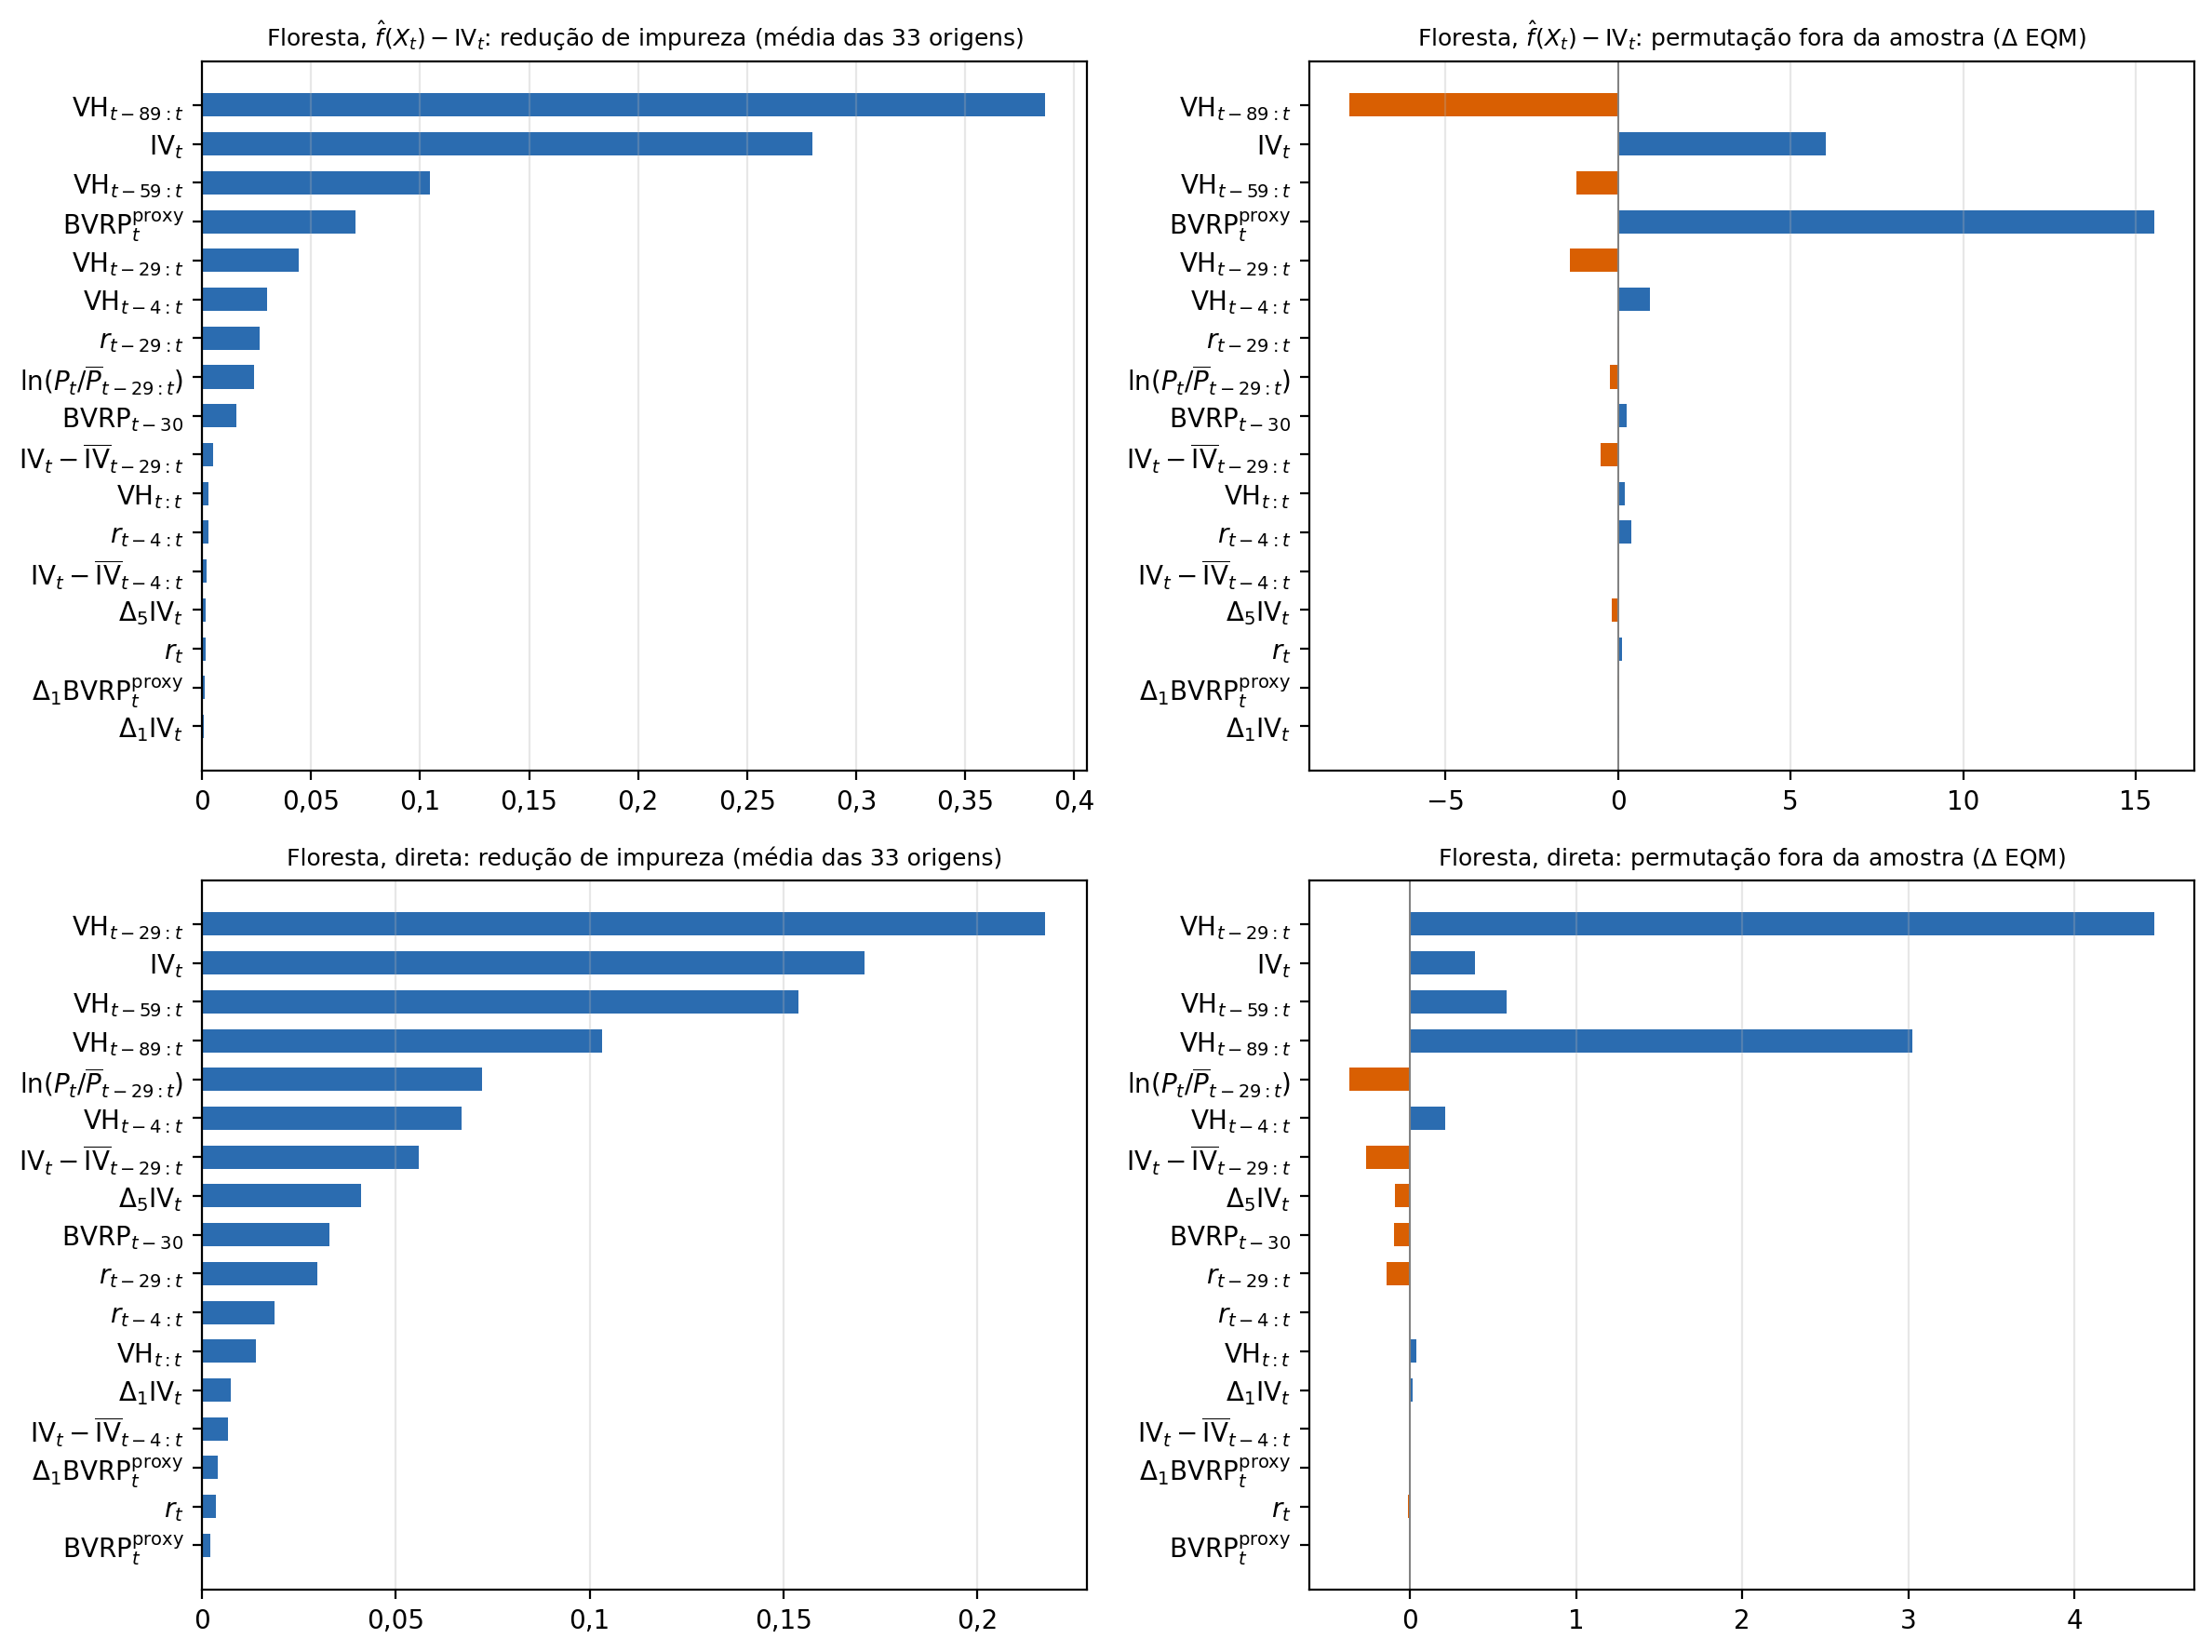
\includegraphics[width=\linewidth]{figs/retornos_nao_linear/fig_importancia.png}
    \caption{Importância das variáveis nas duas formas da floresta: redução de impureza dentro da amostra (média das 33 origens) e aumento do erro quadrático médio do BVRP previsto fora da amostra quando a variável é permutada (barras laranja: permutar reduz o erro).}
    \label{fig:retnl-importancia}
\end{figure}
}{}

A Figura~\ref{fig:retnl-cortes} mostra onde as árvores cortam as
volatilidades. Na forma direta, a floresta corta a VH de 30 dias entre 55\% e
58\% a.a. (mediana ponderada de 56,1\%), e nenhuma redução de impureza vem de
cortes entre 35\% e 40\%. Na forma $\hat f(X_t) - \text{IV}_t$, a VH de 30
dias aparece em 23 das 33 origens, com cortes entre 45\% e 49\% (mediana
ponderada de 48,5\%), e a redução de impureza se concentra na VH de 90 dias,
com cortes entre 60\% e 63\%, e na de 60 dias, perto de 63\%. As árvores
cortam a VH de 30 dias entre 45\% e 58\% a.a., não em $37{,}3\%$: na ponta de
cima ou acima da faixa do corte reestimado em cada origem (de 27,0\% a
51,5\%), e preferem as volatilidades de 60 e de 90 dias à de 30. Os dois regimes da
Seção~\ref{sec:dados-regimes} separam os dias calmos dos demais; os cortes da
floresta separam a volatilidade alta da muito alta.

\IfFileExists{figs/retornos_nao_linear/fig_cortes.png}{
\begin{figure}[H]
    \centering
    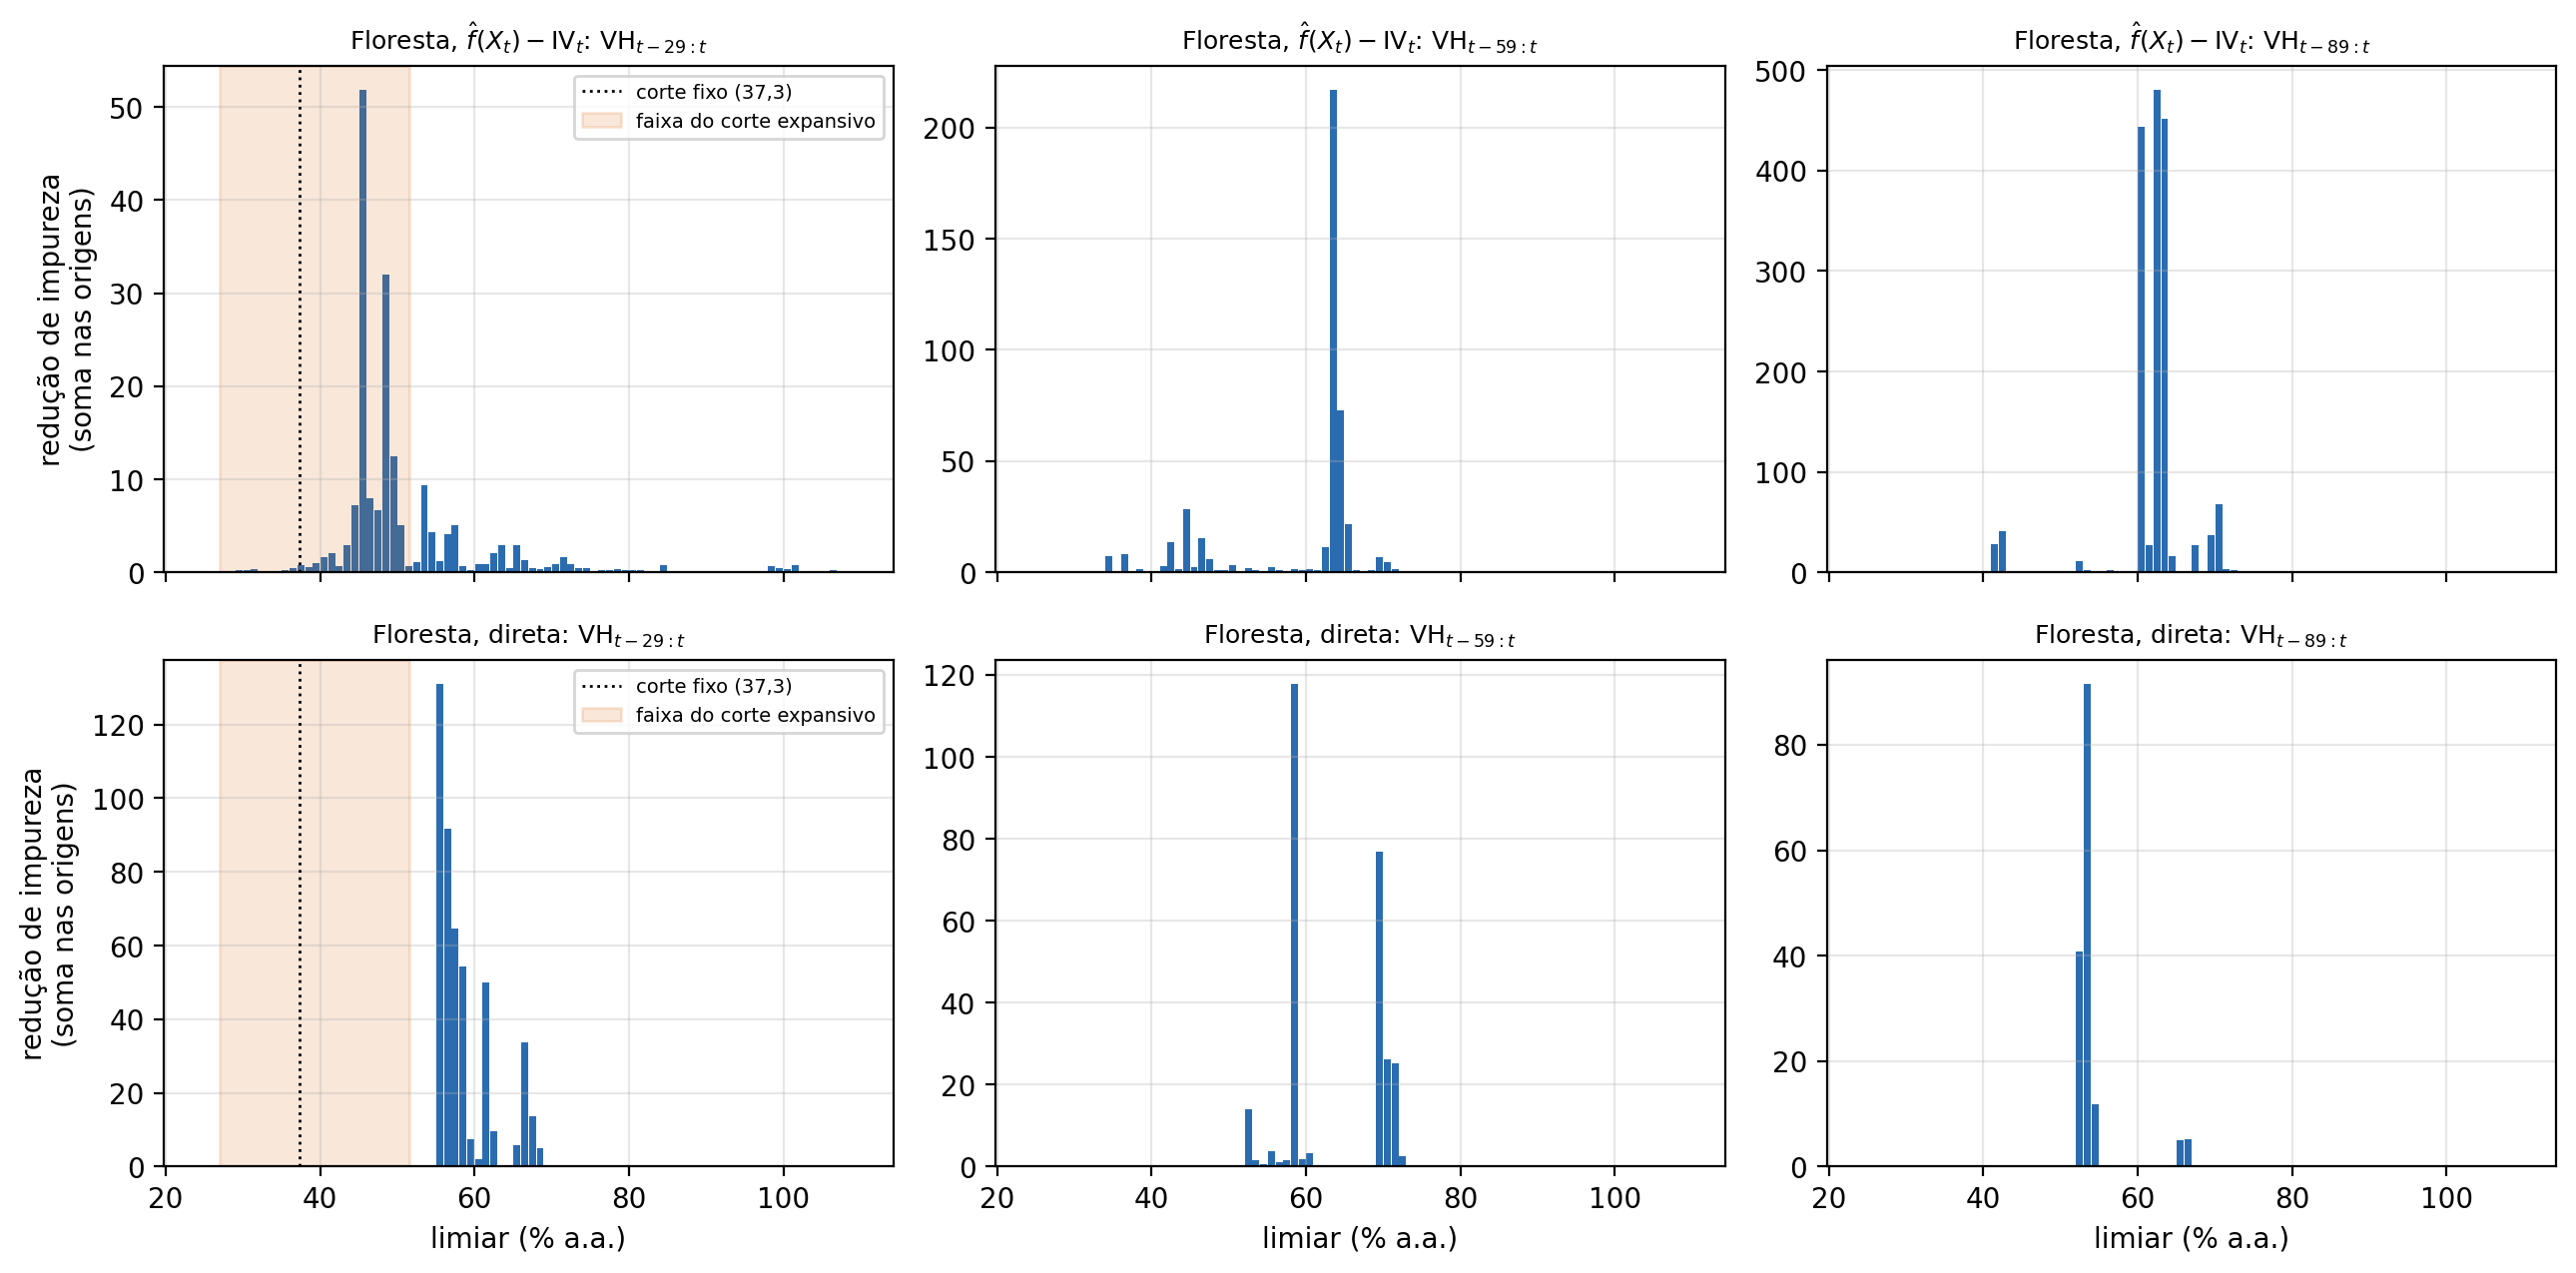
\includegraphics[width=\linewidth]{figs/retornos_nao_linear/fig_cortes.png}
    \caption{Limiares escolhidos pelas árvores nas volatilidades históricas de 30, 60 e 90 dias, nas duas formas da floresta: redução de impureza por faixa de 1 p.p., somada nas 33 origens. Na VH de 30 dias, a linha pontilhada marca o corte fixo de $37{,}3\%$ a.a., e a faixa sombreada, o intervalo do corte reestimado em cada origem.}
    \label{fig:retnl-cortes}
\end{figure}
}{}

A dependência parcial do BVRP previsto na VH de 30 dias
(Figura~\ref{fig:retnl-dependencia}) é plana na maior parte do intervalo e, na
forma direta, cai de 1 a 3 p.p. acima de cerca de 55\%: com a volatilidade
histórica alta, a floresta prevê um prêmio mais negativo, isto é, uma
volatilidade futura mais abaixo da IV. Na forma
$\hat f(X_t) - \text{IV}_t$, o maior salto varia entre as origens.

\IfFileExists{figs/retornos_nao_linear/fig_dependencia_parcial.png}{
\begin{figure}[H]
    \centering
    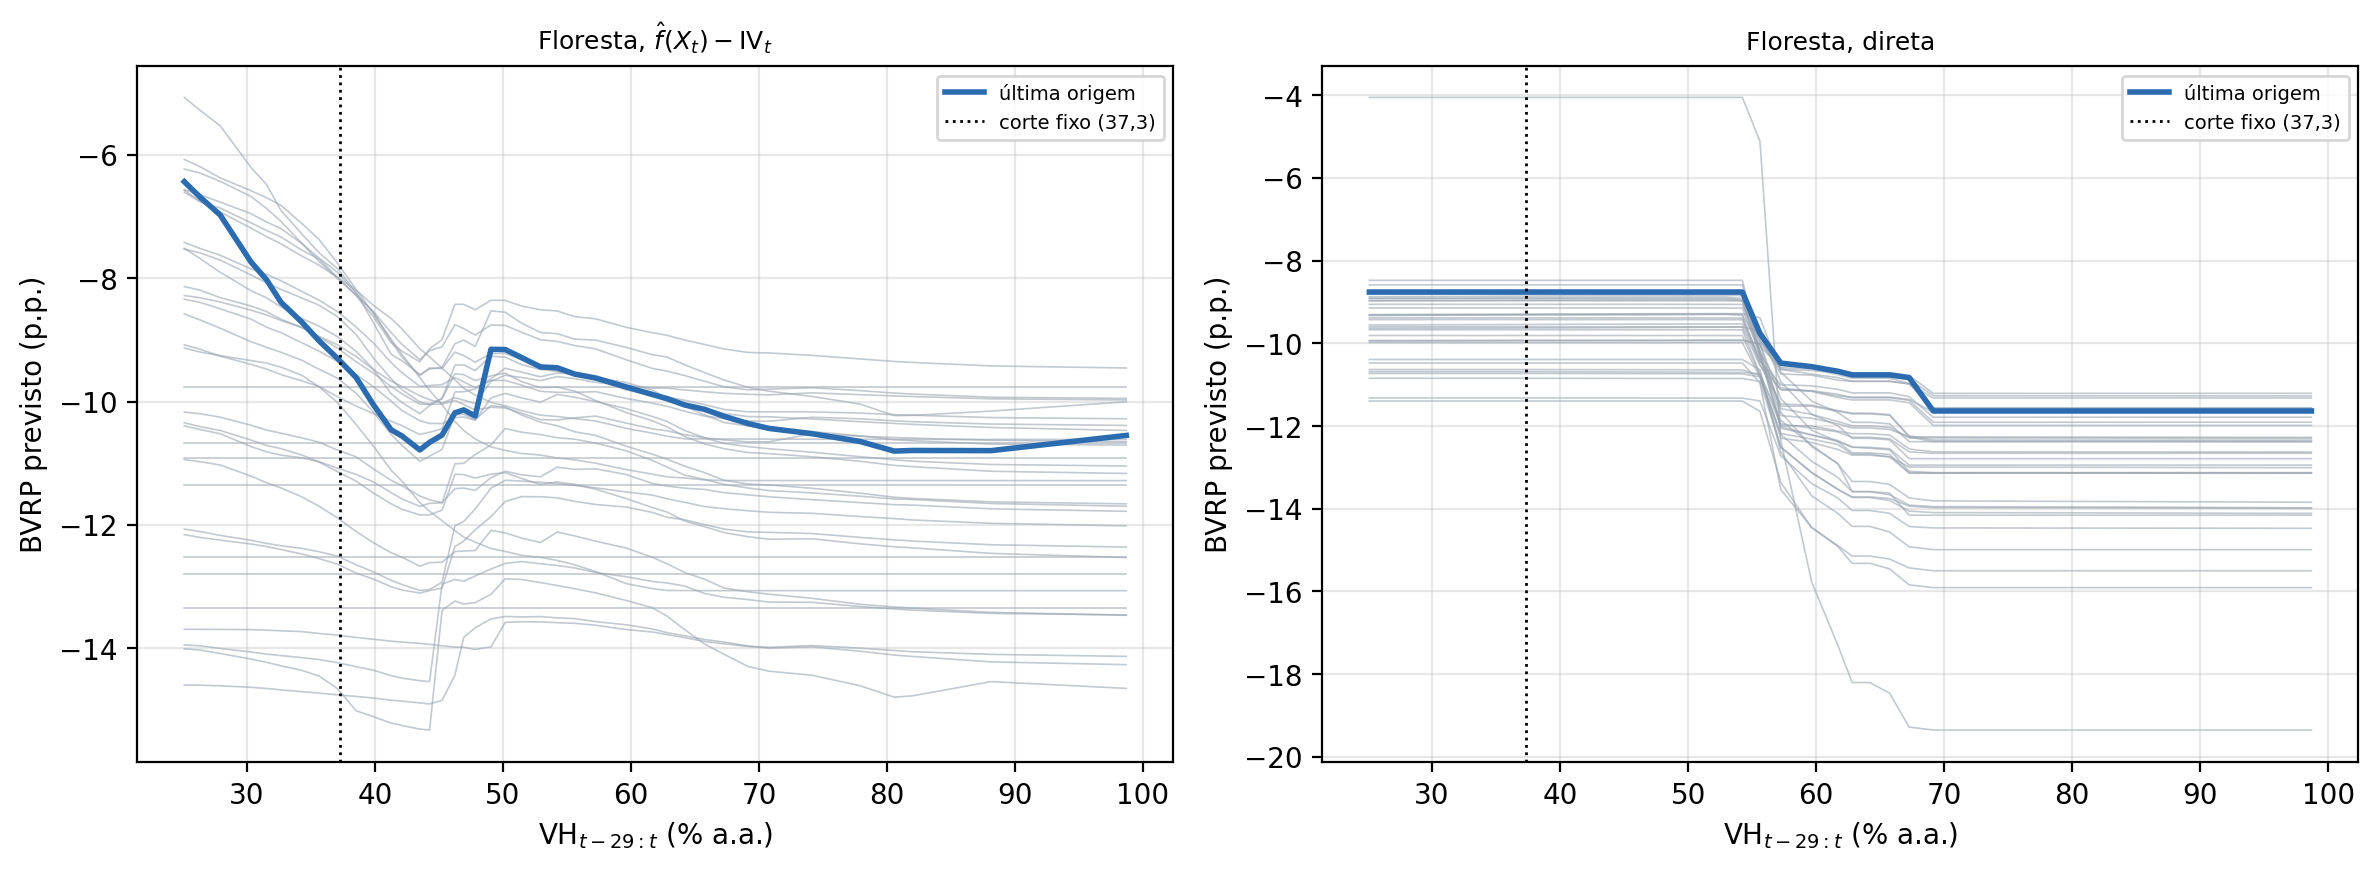
\includegraphics[width=\linewidth]{figs/retornos_nao_linear/fig_dependencia_parcial.png}
    \caption{Dependência parcial do BVRP previsto na volatilidade histórica de 30 dias, nas duas formas da floresta, com a $\text{BVRP}^{\text{proxy}}_t$ recalculada a cada valor da VH. Linhas cinza: as 33 origens; linha azul: a última origem.}
    \label{fig:retnl-dependencia}
\end{figure}
}{}

% =========================================================
\section{Regime de volatilidade e retornos}
\label{sec:retnl-regime}

O teste de significância conjunta também é aplicado por horizonte, com a
variável indicadora do regime de alta volatilidade e sua interação com o BVRP
previsto, como na equação~\eqref{eq:met-retorno-regime}
(Tabela~\ref{tab:retnl-regime}). Para a forma principal, o teste dos três
coeficientes tem valores-$p$ entre 0,36 e 0,89 com o corte fixo e entre 0,42
e 0,73 com o corte expansivo. Nos quatro regressores, só 3 das 48
combinações de regressor, corte e horizonte ficam abaixo do limite de
Bonferroni, sem padrão: o Ridge direto em $h = 60$, com os dois cortes, e a
floresta direta em $h = 20$, só com o corte expansivo. A diferença entre os
regimes continua sugestiva e frágil, como no
Capítulo~\ref{chap:retornos_linear}, e esses valores-$p$ são do HAC, que
ignora a estimação do BVRP previsto.

\begin{table}[H]
\centering
\small
\caption{Teste de significância conjunta por horizonte, com o regime de volatilidade.}
\label{tab:retnl-regime}
\begin{tabular}{rrrrrrr}
\toprule
 & \multicolumn{3}{c}{Corte fixo} & \multicolumn{3}{c}{Corte expansivo} \\ \cmidrule(lr){2-4}\cmidrule(lr){5-7}
$h$ & $\chi^2(3)$ & $p$ & $p$ (regime) & $\chi^2(3)$ & $p$ & $p$ (regime) \\
\midrule
1 & 1{,}36 & 0{,}716 & 0{,}694 & 1{,}30 & 0{,}729 & 0{,}689 \\
5 & 3{,}23 & 0{,}357 & 0{,}203 & 2{,}81 & 0{,}422 & 0{,}249 \\
10 & 3{,}19 & 0{,}363 & 0{,}226 & 2{,}34 & 0{,}505 & 0{,}350 \\
20 & 2{,}70 & 0{,}441 & 0{,}336 & 1{,}86 & 0{,}602 & 0{,}497 \\
30 & 1{,}90 & 0{,}593 & 0{,}522 & 1{,}64 & 0{,}651 & 0{,}549 \\
60 & 0{,}65 & 0{,}886 & 0{,}728 & 1{,}51 & 0{,}680 & 0{,}478 \\
\bottomrule
\end{tabular}
\par\smallskip
\parbox{0.95\linewidth}{\footnotesize\textit{Nota}: $R_{t+h} = \alpha_h + \beta_h\,\widehat{\text{BVRP}}_t + \delta_h D_t + \gamma_h D_t\,\widehat{\text{BVRP}}_t + \varepsilon_{t+h}$, com o BVRP previsto da Tabela~\ref{tab:retnl-principal}. $\chi^2(3)$ e $p$: Wald de $\beta_h = \delta_h = \gamma_h = 0$; $p$ (regime): Wald de $\delta_h = \gamma_h = 0$. HAC com $h+1$ defasagens, que ignora a estimação do BVRP previsto. Corte fixo: $37{,}3\%$ a.a.; expansivo: reestimado em cada origem.}
\end{table}


A Tabela~\ref{tab:retnl-retorno-regime} descreve o retorno futuro médio por
regime, sem o BVRP previsto. Com o corte fixo, o retorno médio é menor no
regime de alta volatilidade em todos os horizontes, de $-0{,}03$ p.p. em
$h = 1$ a $-3{,}23$ p.p. em $h = 30$, e continua menor em $h = 60$
($-2{,}45$ p.p.). Só com a volatilidade extrema, definida pelo quartil
superior da VH com os dados disponíveis até $t$, os retornos ficam perto de
zero ou negativos de $h = 10$ a $h = 30$ e superam os das demais datas em
$h = 60$ ($11{,}46\%$ contra $7{,}64\%$), um padrão de reversão à média.
Nenhuma diferença é significante (valores-$p$ entre 0,20 e 0,82 nas duas
definições), e as 64 datas de volatilidade extrema formam só quatro episódios
(março e abril de 2024, agosto de 2024, março de 2025 e fevereiro e março de
2026).

\begin{table}[H]
\centering
\small
\caption{Retorno futuro médio por regime de volatilidade.}
\label{tab:retnl-retorno-regime}
\begin{tabular}{rrrrr}
\toprule
$h$ & Baixa / demais & Alta / extrema & Diferença & $p$ \\
\midrule
\multicolumn{5}{l}{\textit{Corte fixo ($37{,}3\%$ a.a.)}: Baixa, $N = 394$; Alta, $N = 1{.}382$} \\
1 & 0{,}09 & 0{,}06 & $-$0{,}03 & 0{,}821 \\
5 & 0{,}51 & 0{,}23 & $-$0{,}28 & 0{,}674 \\
10 & 1{,}03 & 0{,}43 & $-$0{,}60 & 0{,}663 \\
20 & 2{,}54 & 0{,}77 & $-$1{,}77 & 0{,}524 \\
30 & 4{,}40 & 1{,}17 & $-$3{,}23 & 0{,}435 \\
60 & 6{,}44 & 3{,}99 & $-$2{,}45 & 0{,}693 \\
\addlinespace
\multicolumn{5}{l}{\textit{Quartil superior em janela expansiva}: Demais, $N = 983$; Extrema, $N = 64$} \\
1 & 0{,}11 & 0{,}38 & 0{,}27 & 0{,}451 \\
5 & 0{,}59 & 0{,}29 & $-$0{,}30 & 0{,}729 \\
10 & 1{,}21 & $-$0{,}02 & $-$1{,}23 & 0{,}287 \\
20 & 2{,}53 & $-$0{,}29 & $-$2{,}82 & 0{,}197 \\
30 & 3{,}82 & 0{,}50 & $-$3{,}32 & 0{,}281 \\
60 & 7{,}64 & 11{,}46 & 3{,}82 & 0{,}521 \\
\bottomrule
\end{tabular}
\par\smallskip
\parbox{0.95\linewidth}{\footnotesize\textit{Nota}: Retorno simples médio de $t$ a $t+h$, em \%. Diferença: regime de alta (ou volatilidade extrema) menos o outro grupo, estimada pela regressão do retorno numa indicadora do regime, com HAC de $h+1$ defasagens. Corte fixo: amostra de modelagem, 23/04/2021 a 03/03/2026. Quartil superior: $\text{VH}_{t-29:t}$ acima do terceiro quartil da própria série com dados até $t$, a partir de 730 observações (22/04/2023 a 03/03/2026).}
\end{table}


% =========================================================
\section{Floresta direto no retorno}
\label{sec:retnl-arvore-retorno}

Uma alternativa às duas etapas é a floresta aplicada direto ao retorno,
$R_{t+h} = g_h(X_t) + \varepsilon_{t+h}$, com uma floresta por horizonte e as
mesmas variáveis e origens, que escolhe as quebras sem passar pelo BVRP
(Tabela~\ref{tab:retnl-arvore-retorno}). O $R^2_{\text{fora}}$ contra a média
histórica do retorno fica entre $-0{,}358$ e $0{,}021$, e nenhum horizonte é
significante no Clark--West (valores-$p$ entre 0,11 e 0,94). Em $h = 60$, a
floresta erra mais que a média histórica (Diebold--Mariano, $p = 0{,}014$). O
$R^2$ dentro da amostra cresce com o horizonte, de 0,02 a 0,39, enquanto o de
fora fica negativo: com alvos de $h$ dias sobrepostos, a floresta se ajusta ao
ruído dos horizontes longos.

\begin{table}[H]
\centering
\small
\caption{Floresta aleatória direto no retorno futuro.}
\label{tab:retnl-arvore-retorno}
\begin{tabular}{rrrrr}
\toprule
$h$ & $R^2_{\text{fora}}$ & $p$ (CW) & $p$ (DM) & $R^2$ dentro \\
\midrule
1 & 0{,}001 & 0{,}133 & 0{,}850 & 0{,}02 \\
5 & $-$0{,}001 & 0{,}186 & 0{,}964 & 0{,}03 \\
10 & 0{,}000 & 0{,}196 & 0{,}997 & 0{,}04 \\
20 & 0{,}021 & 0{,}108 & 0{,}758 & 0{,}07 \\
30 & $-$0{,}075 & 0{,}197 & 0{,}549 & 0{,}15 \\
60 & $-$0{,}358 & 0{,}935 & 0{,}014 & 0{,}39 \\
\bottomrule
\end{tabular}
\par\smallskip
\parbox{0.95\linewidth}{\footnotesize\textit{Nota}: $R_{t+h} = g_h(X_t) + \varepsilon_{t+h}$, com $g_h$ uma floresta aleatória por horizonte, as mesmas variáveis, origens e janela expansiva, e embargo de $h$ dias; 987 previsões. $R^2_{\text{fora}}$ contra a média histórica do retorno; Clark--West unilateral e Diebold--Mariano bilateral contra a média histórica, com HAC de $h+1$ defasagens. $R^2$ dentro: média nas 33 origens.}
\end{table}


% =========================================================
\section{Sinal do retorno}
\label{sec:retnl-sinal}

Em ações, a volatilidade aumenta mais depois de quedas de preço que depois de
altas, o efeito alavancagem \citep{black1976studies, christie1982stochastic}.
No câmbio, o sinal do retorno depende da moeda de cotação --- a queda de uma
moeda é a alta da outra ---, e não há uma direção que corresponda à queda do
ativo. \citet{hansen2005forecast} mostram que, no câmbio marco--dólar, modelos
com efeito alavancagem não superam o GARCH(1,1), ao contrário do que ocorre
com as ações da IBM.

A Tabela~\ref{tab:retnl-sinal} divide a amostra de modelagem pelo sinal do
log-retorno do dia. O BVRP médio é praticamente o mesmo nos dias de alta e de
queda ($-9{,}00$ e $-8{,}63$ p.p.; $p = 0{,}56$). A IV, porém, responde ao
sinal como nas ações: sobe, em média, 0,41 p.p. nos dias de queda e cai 0,46
p.p. nos de alta. A regressão da variação diária da IV nas partes positiva e
negativa do retorno mostra a assimetria: cada ponto percentual de queda eleva a
IV em 0,77 p.p. ($p < 0{,}001$), e as altas não a movem ($p = 0{,}96$). O sinal
do retorno muda a IV, mas não o prêmio.

\begin{table}[H]
\centering
\small
\caption{BVRP e variação da IV pelo sinal do retorno do dia.}
\label{tab:retnl-sinal}
\begin{tabular}{lrrrr}
\toprule
Variável & $r_t > 0$ & $r_t < 0$ & Diferença & $p$ \\
\midrule
$\text{BVRP}_t$ (p.p.) & $-$9{,}00 & $-$8{,}63 & 0{,}37 & 0{,}564 \\
$\Delta_1\text{IV}_t$ (p.p.) & $-$0{,}46 & 0{,}41 & 0{,}88 & $<$0{,}001 \\
\addlinespace
\multicolumn{5}{l}{$\Delta_1\text{IV}_t$ sobre $r_t^+$ e $r_t^-$: $\hat b^+ = 0{,}005$ ($p = 0{,}958$); $\hat b^- = -0{,}772$ ($p < 0{,}001$)} \\
\multicolumn{5}{l}{Simetria, $b^+ + b^- = 0$: $p < 0{,}001$} \\
\bottomrule
\end{tabular}
\par\smallskip
\parbox{0.95\linewidth}{\footnotesize\textit{Nota}: Amostra de modelagem; 877 dias com $r_t > 0$ e 899 com $r_t < 0$. Diferença: dias de queda menos dias de alta, pela regressão numa indicadora de $r_t < 0$, com HAC de 31 defasagens para o BVRP (alvos de 30 dias sobrepostos) e de 2 para $\Delta_1\text{IV}_t$. Duas últimas linhas: $\Delta_1\text{IV}_t = a + b^+ r_t^+ + b^- r_t^- + u_t$, com $r_t^+ = \max(r_t, 0)$ e $r_t^- = \min(r_t, 0)$ em \%, HAC de 2 defasagens; a simetria é $b^+ = -b^-$.}
\end{table}


% =========================================================
\section{Síntese}
\label{sec:retnl-sintese}

O modelo único em árvore não encontra a previsibilidade que o modelo linear
não encontrou. Com a floresta escolhendo os cortes nas volatilidades, o BVRP
previsto tem coeficiente praticamente nulo em todos os horizontes, e o teste
conjunto não rejeita em nenhuma das formas e modelos; a floresta aplicada
direto ao retorno também não supera a média histórica. As árvores cortam a
VH de 30 dias entre 45\% e 58\% a.a., acima do corte de $37{,}3\%$ entre os
regimes, e preferem as volatilidades de 60 e de 90 dias. A diferença de
retornos entre regimes não é significante em nenhuma definição.
O sinal do retorno do dia move a IV, como nas ações, mas não o prêmio.

A amostra inclui a aprovação dos ETFs de Bitcoin à vista pela SEC, em janeiro
de 2024 (Capítulo~\ref{chap:referencial}). A análise trata o período como um
bloco único; a estabilidade dos parâmetros antes e depois da aprovação não é
testada nesta dissertação.
